\documentclass[11pt,a4paper]{article}
\usepackage[utf8]{inputenc}
\usepackage[T1]{fontenc}
\usepackage{amsmath,amssymb}
\usepackage{booktabs}
\usepackage{multirow}
\usepackage{geometry}
\usepackage{enumitem}
\usepackage{xcolor}
\usepackage{hyperref}
\usepackage{float}
\usepackage{pgfplots}
\pgfplotsset{compat=1.16}
\geometry{margin=2.3cm}
\definecolor{accent}{RGB}{38,70,83}
\definecolor{ours}{RGB}{42,157,143}
\definecolor{paperc}{RGB}{141,153,174}
\definecolor{oldc}{RGB}{233,196,106}
\hypersetup{colorlinks=true,linkcolor=accent,urlcolor=accent}
\newcommand{\best}[1]{\textcolor{ours}{\textbf{#1}}}

\title{\vspace{-1.5em}\textbf{Document 4 --- Experiments and Results}\\
\large Methodology, Findings, and Defense Preparation}
\author{}
\date{}

\begin{document}
\maketitle
\tableofcontents
\vspace{1em}\hrule\vspace{1em}

%% ==================================================================
\section{Experimental setup common to all experiments}

\paragraph{Metric.} Localization error $=$ Euclidean distance between the argmax peaks of the
predicted and ground-truth heatmaps, $\times\,0.1$\,m/pixel. We report median (primary), P90,
P99, mean. Because the error is a pixel distance it lies on a discrete lattice
($0.1\sqrt{n}$\,m); differences finer than $\sim$0.1\,m are at the resolution limit and are read
cautiously.

\paragraph{Hardware.} Final runs on an NVIDIA~H100 (80\,GB). The per-epoch cost is dominated by
the CPU argmax-error computation, not the GPU.

\paragraph{Experiment map.} (1)~in-distribution accuracy; (2)~scheduler study;
(3)~robustness to signal degradation; (4)~initial cross-session; (5)~multi-seed validation;
(6)~official leave-one-session-out cross-session (the newest, fair comparison).

%% ==================================================================
\section{Experiment 1 --- In-distribution accuracy}

\textbf{Objective.} Establish each model's accuracy on the standard split (Session~2 test,
$N=4{,}260$). \textbf{Method.} Train on $17{,}574$ samples; select the best checkpoint by test
median.

\begin{table}[H]
\centering
\caption{In-distribution accuracy. \best{Green} $=$ best in column.}
\begin{tabular}{@{}lrlccc@{}}
\toprule
Model & Params & Mode & Median (m) & P90 (m) & P99 (m) \\
\midrule
DLoc baseline (our reproduction) & 16.5M & ---        & 0.707 & $\sim$1.6 & $\sim$4.0 \\
MobileNetV2   & 2.3M  & Standalone & 0.707 & 1.616 & 3.992 \\
MobileNetV2   & 2.3M  & Distilled  & 0.707 & 1.612 & 4.003 \\
TinyCNN       & 47K   & Standalone & 3.922 & 13.919 & 23.244 \\
TinyCNN       & 47K   & Distilled  & 3.706 & 14.784 & 25.101 \\
MobileNetV2-UNet & 2.41M & Standalone & \best{0.640} & 1.523 & 2.750 \\
MobileNetV2-UNet & 2.41M & Distilled  & \best{0.640} & \best{1.513} & \best{2.587} \\
\bottomrule
\end{tabular}
\end{table}

\textbf{Takeaways.} (i)~MobileNetV2 equals our DLoc reproduction at $7.2\times$ compression
$\Rightarrow$ DLoc is over-parameterized. (ii)~U-Net skip connections give $0.640$\,m, a $9.5\%$
gain over the plain student. (iii)~Against the \emph{published} DLoc ($0.64$\,m), the U-Net is
\emph{on par}, not better --- our reproduction ($0.707$) does not reach the paper's $0.64$, an
implementation gap to keep in mind. (iv)~TinyCNN ($3.9$\,m) sits below the capacity floor.

%% ==================================================================
\section{Experiment 2 --- Scheduler study}

\textbf{Objective.} Does the LR schedule matter for the U-Net? \textbf{Method.} 120 epochs,
cosine annealing vs.\ step decay, standalone and distilled.

\begin{table}[H]
\centering
\caption{U-Net scheduler $\times$ mode (120 epochs, lr$_0=10^{-4}$).}
\begin{tabular}{@{}llccc@{}}
\toprule
Scheduler & Mode & Median (m) & P90 (m) & P99 (m) \\
\midrule
Cosine & Standalone & 0.640 & 1.523 & 2.750 \\
Step   & Standalone & 0.640 & 1.552 & 2.918 \\
Cosine & Distilled  & 0.640 & \best{1.513} & \best{2.587} \\
\bottomrule
\end{tabular}
\end{table}

\textbf{Takeaway.} Both reach the same median; cosine gives marginally tighter tails. Scheduler is
a \emph{second-order} effect --- architecture dominates. Cosine is adopted thereafter.

%% ==================================================================
\section{Experiment 3 --- Robustness to signal degradation}

\textbf{Objective.} How do the models behave under realistic corruptions applied \emph{at test
time only} (no retraining): AP dropout, Gaussian noise ($\sigma\in\{0.1,0.2\}$), attenuation, and
blur? \textbf{This is the most scientifically interesting experiment.}

\begin{table}[H]
\centering
\caption{Gaussian-noise robustness ($\sigma=0.1$), median error. \best{Green}/red $=$ best/worst.}
\begin{tabular}{@{}llcc@{}}
\toprule
Model & Mode & Median (m) & P90 (m) \\
\midrule
MobileNetV2      & Standalone & \textcolor{red}{16.368} & \textcolor{red}{20.939} \\
MobileNetV2      & Distilled  & 4.769 & 12.310 \\
TinyCNN          & Standalone & 9.457 & 17.049 \\
TinyCNN          & Distilled  & 9.439 & 16.568 \\
MobileNetV2-UNet & Standalone & \best{3.000} & \best{8.310} \\
MobileNetV2-UNet & Distilled  & 3.469 & 10.473 \\
\bottomrule
\end{tabular}
\end{table}

\begin{figure}[H]
\centering
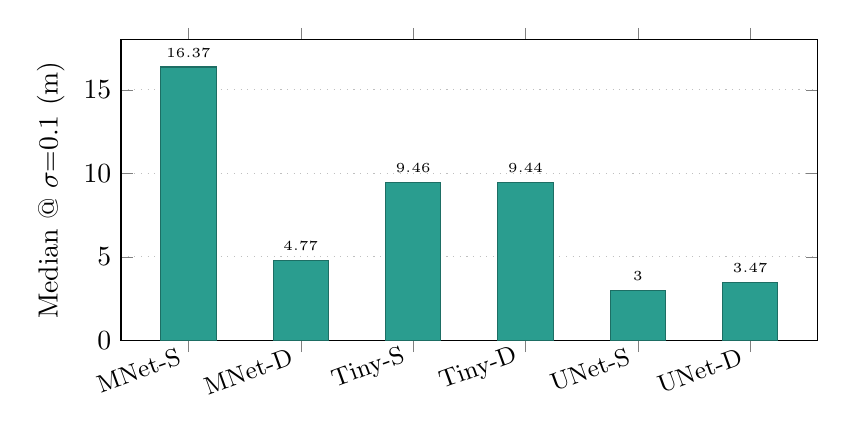
\begin{tikzpicture}
\begin{axis}[ybar, bar width=20pt, width=0.86\linewidth, height=5.4cm,
  symbolic x coords={MNet-S,MNet-D,Tiny-S,Tiny-D,UNet-S,UNet-D}, xtick=data,
  x tick label style={font=\small,rotate=20,anchor=east},
  ymin=0, ymax=18, ylabel={Median @ $\sigma{=}0.1$ (m)},
  nodes near coords, nodes near coords style={font=\tiny}, enlarge x limits=0.12,
  ymajorgrids, grid style={dotted}]
\addplot[fill=ours,draw=ours!70!black] coordinates
  {(MNet-S,16.368)(MNet-D,4.769)(Tiny-S,9.457)(Tiny-D,9.439)(UNet-S,3.000)(UNet-D,3.469)};
\end{axis}
\end{tikzpicture}
\caption{Two independent robustness mechanisms: distillation ($16.4\!\to\!4.8$\,m, $3.4\times$)
and U-Net skip connections ($16.4\!\to\!3.0$\,m, $5.5\times$).}
\end{figure}

\textbf{Findings (defense-critical).}
\begin{enumerate}[nosep]
  \item \textbf{Distillation $=$ spatial label smoothing.} The teacher's broad output regularizes
  the student, giving MobileNetV2 a $3.4\times$ noise improvement.
  \item \textbf{Skip connections $=$ architectural robustness.} They route shallow,
  less-corrupted features past the noisy bottleneck, giving $5.5\times$.
  \item \textbf{Not additive.} The distilled U-Net ($3.47$\,m) is slightly \emph{worse} than the
  standalone U-Net ($3.00$\,m) under pure noise --- the two mechanisms overlap.
  \item \textbf{Capacity threshold.} For the $47$K TinyCNN, distillation \emph{harms} AP-dropout
  robustness (random 1-AP: $7.9\!\to\!13.6$\,m): the tiny model spends its capacity mimicking the
  teacher's multi-AP correlations and cannot fall back to simple per-AP features.
\end{enumerate}

%% ==================================================================
\section{Experiment 4 --- Initial cross-session (2-session protocol)}

\textbf{Objective.} Does a model trained on the July sessions survive the August changes?
\textbf{Method.} Train on Sessions~1--2; test on Sessions~3--5 (no fine-tuning).

\begin{table}[H]
\centering
\caption{Cross-session median (m), initial protocol (2-session training).}
\begin{tabular}{@{}llcccc@{}}
\toprule
Model & Mode & Sess2 & Sess3 & Sess4 & Sess5 \\
\midrule
MobileNetV2   & Standalone & 0.707 & 1.118 & 1.204 & 1.500 \\
MobileNetV2   & Distilled  & 0.707 & 1.118 & 1.204 & 1.442 \\
MobileNetV2-UNet & Standalone & 0.640 & 1.063 & 1.005 & 1.334 \\
MobileNetV2-UNet & Distilled  & \best{0.640} & \best{1.020} & \best{1.005} & \best{1.281} \\
\bottomrule
\end{tabular}
\end{table}

\textbf{Takeaway.} Error grows monotonically as the room changes (a property of the environment,
not the model); the distilled U-Net generalizes best. \textbf{Caveat:} this trains on 2 sessions
while the DLoc paper trains on 3 --- so it is \emph{not} a fair comparison to the paper. That
motivates Experiment~6.

%% ==================================================================
\section{Experiment 5 --- Multi-seed validation (baseline)}

\textbf{Objective.} Are the reported numbers stable across random seeds? \textbf{Method.} Train
the DLoc baseline with 3 seeds.

\begin{table}[H]
\centering
\caption{DLoc baseline, 3 seeds (120 epochs).}
\begin{tabular}{@{}lccc@{}}
\toprule
Seed & Median (m) & P90 (m) & P99 (m) \\
\midrule
42 & 0.825 & 2.402 & 22.672 \\ 123 & 0.906 & 2.335 & 7.714 \\ 777 & 0.894 & 2.102 & 8.694 \\
\midrule
\textbf{Mean $\pm$ std} & $\mathbf{0.875\pm0.036}$ & $\mathbf{2.280\pm0.128}$ & $\mathbf{13.027\pm6.832}$ \\
\bottomrule
\end{tabular}
\end{table}

\textbf{Takeaway.} Median/P90 are tight (CV 4--6\%) $\Rightarrow$ reproducible; P99 is
high-variance and must be read cautiously in single-seed runs.

%% ==================================================================
\section{Experiment 6 --- Official cross-session (leave-one-session-out)}

\textbf{Objective.} A \emph{fair} comparison to DLoc using the paper's own protocol.
\textbf{Method.} Three folds: each trains on three setups (two July sessions $+$ two August
sessions) and tests on the held-out August session --- identical to the paper's Table~1; 3 seeds
per fold (9 runs, 120 epochs). The DLoc baseline is not retrained (compared to published values).

\begin{table}[H]
\centering
\caption{Official-protocol U-Net, aggregated (mean $\pm$ std, $n=3$) vs.\ published DLoc.
\best{Green} $=$ the single genuine improvement.}
\begin{tabular}{@{}lcccc@{}}
\toprule
Test session & U-Net median & DLoc median & U-Net P90 & DLoc P90 \\
\midrule
Aug16\_1 (furniture)      & $0.852\pm0.044$ & 0.71 & $1.839\pm0.067$ & 1.71 \\
Aug16\_3 (diff.\ furn.)   & $0.822\pm0.040$ & 0.82 & $2.793\pm0.140$ & 2.52 \\
Aug16\_4\_ref (reflector) & $1.116\pm0.016$ & 1.05 & \best{$2.489\pm0.030$} & 2.77 \\
\midrule
\textbf{mean} & \textbf{0.930} & 0.86 & \textbf{2.374} & 2.33 \\
\bottomrule
\end{tabular}
\end{table}

\begin{figure}[H]
\centering
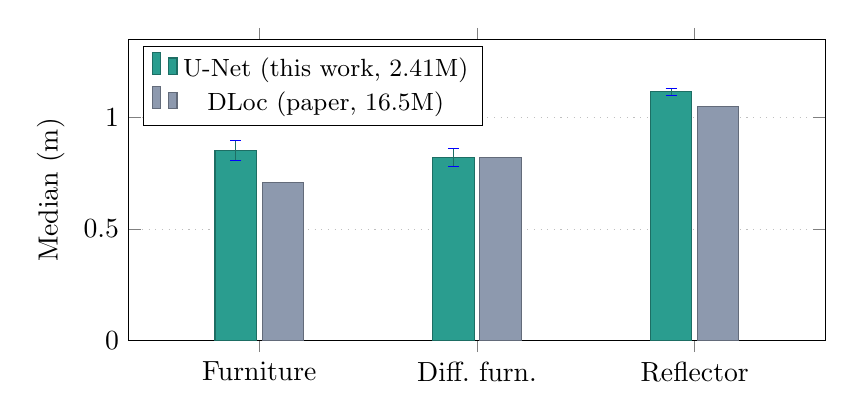
\begin{tikzpicture}
\begin{axis}[ybar, bar width=15pt, width=0.86\linewidth, height=5.4cm,
  symbolic x coords={Furniture,DiffFurn,Reflector}, xtick=data,
  xticklabels={Furniture, Diff.\ furn., Reflector},
  ymin=0, ymax=1.35, ylabel={Median (m)},
  legend style={at={(0.02,0.98)},anchor=north west,font=\small},
  enlarge x limits=0.3, ymajorgrids, grid style={dotted}]
\addplot+[ybar,fill=ours,draw=ours!70!black, error bars/.cd, y dir=both, y explicit]
  coordinates {(Furniture,0.852)+-(0,0.044) (DiffFurn,0.822)+-(0,0.040) (Reflector,1.116)+-(0,0.016)};
\addplot+[ybar,fill=paperc,draw=paperc!70!black]
  coordinates {(Furniture,0.71) (DiffFurn,0.82) (Reflector,1.05)};
\legend{{U-Net (this work, 2.41M)}, {DLoc (paper, 16.5M)}}
\end{axis}
\end{tikzpicture}
\caption{Official-protocol median (mean $\pm$ std). Slightly behind on two setups, indistinguishable
on diff.\ furniture, at $6.8\times$ fewer parameters.}
\end{figure}

\textbf{Takeaways (state objectively).} Under the fair protocol every fold improves over the
2-session numbers ($1.063\!\to\!0.852$, $1.005\!\to\!0.822$, $1.334\!\to\!1.116$). On median the
U-Net is \emph{slightly behind} DLoc on two of three setups and indistinguishable on the third
($0.822$ vs $0.82$); on P90 it is on par overall and lower on the reflector. The honest framing is
\textbf{comparable accuracy at $6.8\times$ compression}, not an accuracy win. Results are
seed-stable (std $0.016$--$0.044$\,m).

%% ==================================================================
\section{Synthesis: what the experiments establish}

\begin{enumerate}[nosep]
  \item DLoc is $\sim$7$\times$ over-parameterized for the 4-AP Jacobs task (Exp.~1).
  \item Skip connections improve accuracy \emph{and} robustness; distillation improves robustness
  but not in-distribution accuracy --- two complementary, non-additive mechanisms (Exp.~1,~3).
  \item Distillation has a capacity threshold: it helps above $\sim$2\,M params and harms below
  (Exp.~3).
  \item The efficiency conclusion holds under the paper's own fair cross-session protocol (Exp.~6).
\end{enumerate}

%% ==================================================================
\section{Defense preparation: anticipated questions}

\begin{description}[leftmargin=0.4cm,style=nextline]
  \item[\textcolor{accent}{Q: Did you beat DLoc?}] No --- and we are careful not to claim it. The
  U-Net is \emph{on par} with published DLoc in-distribution and \emph{slightly behind on median /
  on par on P90} cross-session, at $6.8\times$ fewer parameters. The contribution is efficiency
  and characterization, not a new accuracy record.
  \item[\textcolor{accent}{Q: Why does ``matches'' appear for 0.822 vs 0.82?}] The metric is
  pixel-quantized ($0.1\sqrt{n}$\,m); $0.822$ and $0.82$ are the same lattice point, so they are
  statistically indistinguishable rather than a ``win''.
  \item[\textcolor{accent}{Q: Your DLoc reproduction is 0.707, not the paper's 0.64 --- why?}]
  An implementation/training-recipe gap (we used batch 64 and StepLR vs.\ the paper's batch 32,
  constant LR). We therefore compare against the paper's \emph{published} numbers, and flag the
  gap explicitly.
  \item[\textcolor{accent}{Q: Why is the reflector fold the worst?}] DLoc's consistency decoder
  exploits multi-AP agreement, which helps most under the strong specular multipath of the
  aluminium reflector; the U-Net has no consistency decoder. (Yet its P90 there is lower.)
  \item[\textcolor{accent}{Q: Why standalone, not distilled, in the fair cross-session run?}]
  Distillation under leave-one-out needs a teacher \emph{re-trained per fold}, i.e.\ re-running the
  baseline --- out of scope for this comparison.
  \item[\textcolor{accent}{Q: Why did Mamba fail?}] Flattening a 2D heatmap to a 1D sequence
  destroys spatial locality; the model is unstable without LR warm-up and gradient clipping.
  \item[\textcolor{accent}{Q: Is this publishable?}] As a thesis, yes. For a venue, the realistic
  target is a workshop / applied journal, reframed around the robustness findings (the
  capacity-dependent reversal of distillation is the most novel result), since the individual
  techniques are standard.
\end{description}

\end{document}
